\documentclass[reprint,amsmath,amssymb,aps,pra]{revtex4-2}

\usepackage{graphicx}
\usepackage{dcolumn}
\usepackage{bm}
\usepackage{hyperref}% add hypertext capabilities
%\usepackage[mathlines]{lineno}% Enable numbering of text and display math
%\linenumbers\relax % Commence numbering lines
\usepackage{braket}
\usepackage{physics}
\usepackage{amsmath}
\usepackage{amssymb}
\usepackage{tcolorbox}
\usepackage{amsthm}
\usepackage[]{quantikz}
\usepackage[ruled,vlined,linesnumbered]{algorithm2e}
\usepackage{mathdots}

\newtheorem{claim}{Claim}
\newtheorem{proposition}{Proposition}
\newtheorem{observation}{Observation}
\newtheorem{theorem}{Theorem}[section]
\newtheorem{lemma}[theorem]{Lemma}
%\usepackage[showframe,%Uncomment any one of the following lines to test 
%%scale=0.7, marginratio={1:1, 2:3}, ignoreall,% default settings
%%text={7in,10in},centering,
%%margin=1.5in,
%%total={6.5in,8.75in}, top=1.2in, left=0.9in, includefoot,
%%height=10in,a5paper,hmargin={3cm,0.8in},
%]{geometry}

\newcommand{\smallket}[1]{{|{#1}\rangle}}

\begin{document}

% \preprint{APS/123-QED}

\title{A Polylogarithmic-Depth Quantum Multiplier}% Force line breaks with \\
\author{Fred Sun${}^{1,2}$}
% \altaffiliation[Also at ]{University of Waterloo, Waterloo, ON}
\author{Anton Borissov${}^{1}$}
\affiliation{${}^{1}$softwareQ inc.}
\affiliation{${}^{2}$University of Waterloo}

\newcommand{\anton}[1]{{\color{red}(anton): #1}}
\newcommand{\fred}[1]{{\color{blue}(fred): #1}}

\date{\today}
\begin{abstract}
We present a quantum algorithm for multiplying two $n$-bit integers with overall circuit depth and $T$-depth both bounded by $O(\log^{2} n)$, while using $O(n^{2})$ gates and ancillary qubits. Our construction generates partial products via indicator-controlled copying and adds them using a binary adder tree, enabling parallel accumulation with logarithmic depth overhead per level. To the best of our knowledge, our design has the lowest $T$-depth among all multiplication algorithms using the Clifford + $T$ model. By optimizing both circuit depth and $T$-depth, our construction advances the practical feasibility of large-scale fault-tolerant quantum algorithms.
\end{abstract}

\maketitle
\section{Introduction}
% General discussion of quantum circuits implementing arithmetic and various metrics

Quantum arithmetic is a fundamental building block in many quantum algorithms,
most notably the modular exponentiation component of Shor’s factoring algorithm \cite{Shor1997, pavlidis2013fastquantummodularexponentiation}, but also in scientific
computing applications and numerical approximations, such as Hamiltonian simulations, the HHL algorithm for solving linear systems, and Taylor series approximations \cite{Childs_2017, Harrow_2009, Berry_2015}.
Efficient implementations of elementary arithmetic operations, eg. addition and
multiplication, play a critical role in the optimization of large-scale quantum
circuits. 
\cite{wang2024comprehensivestudyquantumarithmetic,
cuccaro2004newquantumripplecarryaddition,
Draper2004, Ruiz_Perez_2017,
gidney2025classicalquantumadderconstantworkspace}.

In fault-tolerant quantum computing, the cost of an algorithm is more accurately
captured by circuit depth and, in particular, by $T$-depth, rather than
by total gate count alone \cite{Selinger2013,Amy2012}. Since non-Clifford gates
dominate the overhead of fault-tolerant implementations, optimizing $T$-depth is
often more desirable for practical performance, even at the expense of qubit
count or Clifford gate depth.

In this work, we study the multiplication of two $n$-bit natural numbers. We present a simple and modular quantum multiplication algorithm
that achieves $O(\log^2 n)$ depth and $T$-depth, making it the fastest known
multiplication circuit constructed entirely from standard Clifford+$T$
primitives. The algorithm prioritizes minimizing $T$-depth and overall depth, trading off a
quadratic number of clean ancillary qubits and T-gates to achieve these performance
improvements. 

\subsection{Related Work}

\begin{table*}[t]
    \centering
    \caption{Asymptotic resource costs for quantum multiplication algorithms.}
    \begin{tabular}{|c|c|c|c|}
    \hline
        Paper & $T$-depth & $T$-count & Ancillary Qubit Count\\\hline
        Shift-and-Add \cite{Munoz-Coreas2019} 
        & $O(n^2)$  
        & $O(n^2)$ 
        & $O(n)$\\\hline
        Karatsuba \cite{parent2017improvedreversiblequantumcircuits} 
        & $O(n^{1.158})$ 
        & $O(n^{\log_2 3})$ 
        & $O(n^{1.427})$\\\hline
        Toom--Cook \cite{Putranto2023} 
        & $O(n^{1.0569})$ 
        & $O(n^{\log_8 15})$ 
        & $O(n^{1.245})$\\\hline
        Schönhage--Strassen$^{*}$ \cite{Nie2023}
        & $O(\log^2 n)$  
        & $O(n\log n\log\log n)$ 
        & $O(n\log n\log\log n)$\\\hline
        \textbf{This work} 
        & $O(\log^2 n)$  
        & $O(n^2)$ 
        & $O(n^2)$\\\hline
    \end{tabular}\\
    \footnotesize
    $^{*}$The quantum Schönhage--Strassen algorithm is a galactic algorithm and requires the input size to be $n \geq 2^{40}$ \cite{Nie2023}.
    
    \label{table:compare_asymp}
\end{table*}

\begin{table*}[t]
    \centering
    \caption{Concrete (non-asymptotic, tight upper-bounded) resource costs for quantum multiplication algorithms. `--' indicates no concrete metric was provided.}
    \resizebox{\textwidth}{!}{
        \renewcommand{\arraystretch}{1.2}

    \begin{tabular}{|c|c|c|c|c|c|}
    
    \hline
        Paper 
        & Depth 
        & Toffoli Depth 
        & Toffoli Count 
        & Gate Count 
        & Ancillary Qubits
        \\
    \hline
        Shift-and-Add \cite{Munoz-Coreas2019} 
        & $5n^2+2n-6$ 
        & $3n^2-14$ 
        & $3n^2-14$ 
        & $7n^2-4n+4$ 
        & $2n+1$
        \\
    \hline
        Karatsuba \cite{parent2017improvedreversiblequantumcircuits} 
        & -- 
        & $\approx n^{1.158}$ 
        & $98n^{\log 3}$ 
        & $218n^{\log{3}}$ 
        & $\approx n^{1.427}$
         \\
    \hline
        Toom--Cook \cite{Putranto2023} 
        & -- 
        & $\approx n^{1.0569}$ 
        & $112n^{\log_8 15}-128n$ 
        & -- 
        & $\approx n^{1.245}$
         \\
    \hline
        Schönhage--Strassen (weaker) \cite{Nie2023} 
        & $58\log^2 n -126\log n+806$ 
        & $58\log^2{n}+O(\log{n})   $  
        & --  
        & -- 
        & $13n^{1.5}+4\log n-8$
         \\
    \hline
        \textbf{This work} 
        & $3\log^2n + 17\log{n} + 20$ 
        & $3\log^2n+7\log{n}+14$ 
        & $12n^2-n\log{n}$ 
        & $26n^2+2n\log{n}$ 
        & $3n^2$
        \\  
    \hline
    \end{tabular}}
    \label{table:compare}
\end{table*}

Many quantum circuits for integer multiplication have been proposed, each with
trade-offs among depth, $T$-count, and ancillary qubit count. In this work, we
compare against representative constructions, as surveyed by Wang et al. \cite{wang2024comprehensivestudyquantumarithmetic}, that serve as benchmarks in
fault-tolerant settings: shift-and-add (schoolbook) multiplication, Karatsuba's
algorithm, Toom–Cook multiplication, and divide-and-conquer approaches such as
the quantum Schönhage–Strassen algorithm
\cite{Munoz-Coreas2019, parent2017improvedreversiblequantumcircuits,
Putranto2023, Nie2023}. The shift-and-add multiplication method, implemented by Muñoz-Coreas \emph{et
al.}, uses Toffoli gates and controlled adders to directly construct the
standard schoolbook multiplication procedure \cite{Munoz-Coreas2019}. This
approach has quadratic $T$-depth and $T$-count, but requires only $O(n)$
ancillary qubits.

The quantum implementations of Karatsuba's algorithm and the Toom--Cook multiplication algorithm reduce asymptotic gate complexity by recursively decomposing large multiplications into smaller subproblems \cite{parent2017improvedreversiblequantumcircuits, Putranto2023}. These approaches improve $T$-count and $T$-depth compared to shift-and-add multiplication at the tradeoff of a greater number of ancillary qubits.


Nie et al. \cite{Nie2023} introduce the quantum Schönhage--Strassen
algorithm, which achieves $O(\log^2 n)$ depth and $O(n\log n\log\log n)$ $T$-count by
employing a recursive structure based on the Fast Fourier Transform. This
algorithm also requires only $O(n\log n\log\log n)$ ancillary qubits. However,
the asymptotic expressions hide extremely large constant factors, making the
approach practical only for very large input sizes ($n \ge 2^{40}$
\cite{Nie2023}). 
This paper also designed a simplified version of the
Schönhage--Strassen algorithm with $O(n^{1.5})$ gate and qubit counts, which has
more manageable coefficients and could be implemented for moderately large
inputs. 

A tree-like solution can be applied to multiplication, using a similar method to their Quantum Carry Lookahead Adder \cite{Draper2004}. It was later proposed that a family of circuits can optimize multiplication down to depth and Toffoli depth $8\log^2{n}+O(\log{n})$ based on the standard textbook multiplication algorithm, such that it conducts addition in the fashion of the binary tree \cite{Nie2023}. However, such a design has both size and number of ancillary qubits $O(n^2)$ and no concrete implementation has yet been provided.

Our algorithm follows this approach to achieve both a depth and Toffoli depth of $3\log^2{n}+O(\log{n})$ through an optimized shift-and-add-based divide-and-conquer structure. In this paper, we also introduce explicit circuit constructions with detailed proofs of correctness and provide concrete (non-asymptotic, tight upper-bounded) resource-cost analyses across all submodules. Furthermore, our approach is optimized to have low constant factors in the resource costs, making it a practical solution to quantum multiplication for when circuit depth is the most important criterion. A summary of our algorithm's resource costs is shown in
Table~\ref{table:compare_asymp} and Table~\ref{table:compare}.

\begin{comment}
Their second result \anton{what second result? (I think the last
sentence, this sentence, and the next two sentences should be rewritten)} is a
parallelized divide-and-conquer strategy. Conceptually, this algorithm follows a
very similar approach to ours and achieves the same asymptotic resource costs,
but with worse constant factors. Furthermore, their analysis contains gaps, and
no explicit circuit construction or detailed proof of correctness is provided.
\anton{perhaps it would be better to highlight the improvements over their paper
(say how great this paper is) rather than say how bad their paper is. You begin to do this in the next paragraph, but that paragraph also needs to be rewritten.}


Our algorithm occupies a distinct point in this design space, achieving
polylogarithmic depth and $T$-depth through an optimized shift-and-add–based
divide-and-conquer structure. Futhermore, our approach avoids excessive constant
factors, making it a practical candidate for near-term fault-tolerant
implementations. 
\end{comment}


The remainder of the paper is organized as follows. In Section~2, we provide the foundations for our algorithm, including the design and analysis of all submodules used. In Section~3, we explicitly provide the full fast quantum multiplication algorithm and explicitly analyze our algorithm's depth, Toffoli depth, size, and ancilla requirements.






\begin{comment}


Quantum arithmetic is a core subroutine in many quantum algorithms \cite{Shor1994}.
In fault-tolerant settings, the cost of an algorithm is better quantified using circuit depth rather than total gate count~\cite{Selinger2013,Amy2012}.

% Structure of the Landscape of quantum circuits implementing multiplication
% Very brief description about each method listed, but then focus on the Schonhage-Strassen approach
% with the goal of explaining our 'competitor's' work in order to help the reader distinguish betweeen
% their work and what we propose.
Quantum circuits implementing multiplication fall into the following classes: 
standard ``schoolbook'',%~\cite{},
Karatsuba/Took-Cook,%~\cite{}/Toom-Cook~\cite{},
QFT-based,%~\cite{},
carry-save,%~\cite{},
divide-and-conquer.%~\cite{}.



% Describe in a high level our approach
Our approach focuses on providing a simple easy-to-understand divide-and-conquer algorithm
that is competitive in terms of reducing the overhead in terms of $T$-depth.

% Introduce notation...

   We would like to perform the operation using a Clifford+T quantum circuit:
\begin{align}
    \ket{x}\ket{y}\ket{0}^{\otimes 2n}\ket{0}^{\otimes N_{anc}}
    \xrightarrow{\quad}
    \ket{x}\ket{y}\ket{xy}\ket{0}^{\otimes N_{anc}},
\end{align}
where we encode $x,y$ and $xy$ into a quantum circuit using the binary representation,
$x = \sum_{i=0}^{n-1}2^ix_i$, 
$y = \sum_{i=0}^{n-1}2^iy_i$,
$xy = \sum_{i=0}^{2n-1}2^iz_i$,
so that
$\ket{x} = \ket{x_{n-1}}\cdots\ket{x_0}$,
$\ket{y} = \ket{y_{n-1}}\cdots\ket{y_0}$,
$\ket{xy} = \ket{z_{2n-1}}\cdots\ket{z_0}$, 
\end{comment}


\section{Preliminaries} \label{sec:prelim}

\subsection{Notation}\label{subsec:math}
Consider two $n$-bit positive integers, $x,y$. We express their binary representation as
\begin{align}
    x &= x_{n-1}\cdot2^{n-1}+\dots+x_1\cdot2+x_0, \label{eq:DefnX}\\
    y &= y_{n-1}\cdot2^{n-1}+\dots+y_1\cdot2+y_0,
\end{align}
where $n = \lfloor\log_2{\max{(x,y)}}\rfloor+1$, and for $0\le i \le n-1$, $x_i,y_i \in \{0,1\}$. The most significant bit of $x$ is $x_{n-1}$ and the least significant bit is $x_0$.

We structure our algorithm around the following representation of the product:
\begin{align}
    xy  &= y_{n-1}(2^{n-1}x)+\dots+y_1(2x)+y_0x. \label{Eq1}
\end{align}
This allows us to think of each $y_i$ as a binary indicator variable for whether
$2^ix$ is included in the sum to compute the product. 

We find it useful to introduce $n$-bit \emph{partial products}, $\alpha^{(0,i)}
:= y_ix$, and we introduce \emph{partial sums} defined as sums of consecutive
partial products weighted with factors of $2$:
\begin{align}
\alpha^{(d,r)} 
= \sum_{k=0}^{2^d-1} 2^k \alpha^{(0,r2^d + k)}
= \left(\sum_{k=0}^{2^d-1} 2^k y_{r2^d + k}\right) x.
% \alpha^{(0,r2^d)}+\dots+2^{(2^d-1)}\alpha^{(0,r2^d+2^d-1)}.
\label{eq:DefnAlpha}
\end{align}
Since it is possible to express $\alpha^{(d,r)}$ as a product of a $2^d$ bit
integer and a $n$ bit integer, for $1 \le d \le \lceil \log{n}\rceil$, each
$\alpha^{(d,r)}$ is a $n+2^d$ bit nonnegative integer.
%
Note that the final partial sum, $\alpha^{(\lceil \log n \rceil, 0)}$,
is the desired product, $xy$.


Throughout the paper, if we have an $m$-bit nonnegative integer, $a = a_{m-1}2^{m-1}+\cdots+a_0$, we shall
encode it into an $m$-qubit register as,
\begin{align}
\ket{a} \equiv 
\ket{a_{m-1}} \cdots \ket{a_{0}}. \label{eq:MbitQubit}
\end{align}

We would like to find an efficient circuit that implements the following transformation,
\begin{align}
    \ket{x}\ket{y}\ket{0}^{\otimes 2n}
    \ket{0}_{anc} \xrightarrow[\qquad]{} \ket{x}\ket{y}\ket{xy}\ket{0}_{anc},
    \label{eq:Desired}
\end{align}
where $\ket{x}$, $\ket{y}$, $\ket{xy}$ represent $n$, and $2n$-qubit
registers, defined using 
Eq.~\eqref{eq:MbitQubit}.
$\ket{0}_{anc}$ represents a helper ancilla register of size that will be determined later.

To implement the above algorithm, it is useful to 
define $n$-qubit registers, $\ket{x^{(i)}}$ and $\ket{y^{(i)}}$, for $i=0,\ldots,n-1$.
% Using Eq.~\eqref{eq:MbitQubit}, 
We shall also use registers $\ket{\alpha^{(d,r)}}$ which have $n+2^d$-qubits for $1 \le d \le \lceil\log n\rceil$.
We also abuse notation by writing $\ket{0^{(i)}}$ to denote either $\ket{x^{(i)}}$ or $\ket{y^{(i)}}$ that is initialized to $\ket{0}^{\otimes n}$.



% We label $\ket{y}$ registers a bit differently. For $n$ copies of register $\ket{y}$, we have $n$ copies of each qubit of $\ket{y}$. We group all $n$ copies of each qubit together, so $\ket{y^{(i)}}$ is a register containing $n$ copies of the $i$th qubit of $\ket{y}$, namely $\ket{y_i}^{\otimes n}$.

% We can combine Equations (1) and (2) as follows:

For the remainder of this section, we describe the three submodules needed to efficiently compute all partial sums, $\ket{\alpha^{(d,r)}}$. 
The final partial sum, with $d=\lceil\log n\rceil$ and $r = 0$, is equal to $\ket{xy}$.


%
% This expression will be further explained in
% Section~\ref{subsec:efficient_adder}

% Now, using Eqs.~\eqref{eq:NbitQubit} and \eqref{eq:DefnAlpha}
% \begin{align}
% \ket{\alpha^{(d,r)}} = \ket{\alpha^{(d-1,2r)} + 2^{2^{(d-1)}}\alpha^{(d-1,2r+1)}}.
% \end{align}
% More explicitly,
% \begin{align}
%     \ket{\alpha^{(d,r)}} = \ket{\alpha^{(0,r2^d)}+\dots+2^{(2^d-1)}\alpha^{(0,r2^d+2^d-1)}}.
% \end{align}
% Consequently, for $d \in [1,\lceil \log{n} \rceil]$, each $\ket{\alpha^{(d,r)}}$ requires $n+2^d$ qubits to store. This expression will be further explained in Section~\ref{subsec:efficient_adder}


% For an $n$-bit unsigned integer $x$, we can represent $2x$ by shifting all bits of $x$ 1 unit to the left. Inductively, $2^ix$ is computed by shifting all bits of $x$ to the left by $i$ positions, requiring at most $n+i$ bits to store.


\begin{comment}
\subsection{Computing All Binary Power Multiples of $x$} \label{subsec:P2M}

The first step of the construction is to compute the values $2^i x$ for all $i \in \{1,2,\dots,n\}$. We refer to the operation that produces $2^i x$ as \emph{copy\_and\_shift}.

\begin{claim}
    $x^{(i)} = 2^i x$ can be computed out-of-place in $O(1)$ depth using an $(n+i)$-qubit ancillary register.
\end{claim}

\begin{proof} 

We represent $\ket{x}$ in the computational basis as $\ket{x_{n-1} \dots x_0}$. The mapping corresponding to multiplication by $2^i$ is 
\[ 
x_{n-1} \dots x_0 \;\longrightarrow\; x_{n-1} \dots x_0 \, \underbrace{0 \cdots 0}_{i}. \] 

This mapping is implemented by applying CNOT gates in parallel from the $k$th qubit of $\ket{x}$ to the $(k+i)$th qubit of an ancillary register, for each $k \in \{1,\dots,n\}$. Each CNOT copies a single computational-basis bit into the appropriately shifted position of the target register.\\

Since all CNOT gates act on disjoint pairs of qubits, they may be executed simultaneously, yielding an overall circuit depth of $O(1)$.

\end{proof}

As an example, the circuit diagram for copy-and-shift($\ket{x^{(0)}}, \ket{x^{(1)}}$, 1) is provided in Fig.~\ref{fig:copyandshift} and a more formal description of the procedure is described in Algorithm~\ref{algo:copyandshift}.\\

\begin{figure}[H]
    \centering
    \resizebox{0.3\columnwidth}{!}{
    \begin{quantikz}[column sep=0.4cm]
    \lstick{${\ket{x^{(1)}_{4}}}$} & \qw & \qw & \qw & \targ & \qw & \qw \\
    \lstick{${\ket{x^{(1)}_{3}}}$} & \qw & \qw & \targ & \qw & \qw & \qw \\
    \lstick{${\ket{x^{(1)}_{2}}}$} & \qw & \targ & \qw & \qw & \qw & \qw \\
    \lstick{${\ket{x^{(1)}_{1}}}$} & \targ & \qw & \qw & \qw & \qw & \qw \\
    \lstick{${\ket{x^{(1)}_{0}}}$} & \qw & \qw & \qw & \qw & \qw & \qw \\[0.35cm]
    \lstick{${\ket{x^{(0)}_{4}}}$} & \qw & \qw & \qw & \qw & \qw & \qw \\
    \lstick{${\ket{x^{(0)}_{3}}}$} & \qw & \qw & \qw & \ctrl{-6} & \qw & \qw \\
    \lstick{${\ket{x^{(0)}_{2}}}$} & \qw & \qw & \ctrl{-6} & \qw & \qw & \qw \\
    \lstick{${\ket{x^{(0)}_{1}}}$} & \qw & \ctrl{-6} & \qw & \qw & \qw & \qw \\
    \lstick{${\ket{x^{(0)}_{0}}}$} & \ctrl{-6} & \qw & \qw & \qw & \qw & \qw
    \end{quantikz}
    }
    \caption{Implementation of $\texttt{copy\_and\_shift}(|x^{(0)}\rangle, |x^{(1)}\rangle, 1)$}
    \label{fig:copyandshift}
\end{figure}

\begin{algorithm}[H]
\label{algo:copyandshift}
\caption{copy\_and\_shift(ctrl, targ, shift)}
\KwIn{\textbf{ctrl}: control register $\ket{x^{(i)}}$, \textbf{targ}: target register, \textbf{shift}: number of bit shifts}
\For{$k \gets i $ \KwTo $i+n-1$ }{
    Apply a CNOT gate controlled from the $k$th qubit of \textit{ctrl}, targeted on the $k+\text{\textit{shift}}$-th qubit of \textit{targ}
}

\end{algorithm}


As noted in Claim 1, each $2^ix$ is computable in constant time. However, computing all such values sequentially would require linear time. To avoid this, we compute all $2^i x$ values in parallel using the procedure described in Algorithm~\ref{algo:twopowermultiples}.

We define a register to be \emph{filled} if it contains a valid value of the form $2^i x$, and \emph{unfilled} otherwise.

\begin{algorithm}[H]
\label{algo:twopowermultiples}
\caption{binary\_power\_multiples}
\KwIn{
$\ket{x^{(0)}}\underbrace{\ket{0^{(1)}}^{\otimes n}\ket{0^{(2)}}^{\otimes n}\dots \ket{0^{(n-1)}}^{\otimes n}}_{n-1}$\\

}
filled $\gets [ \ket{x^{(1)}}]$\;

\For{$t \gets 0$ \KwTo $\lceil{\log_2{n}}\rceil$}{
    \ForEach{$\ket{x^{(i)}} \in$ filled}{
        copy\_and\_shift($\ket{x^{(i)}},\ket{0^{(i+2^t)}},2^t$)\;
        filled.append\_back($\ket{x^{(i+2^t)}}$)\;
    }
}
\end{algorithm}
At iteration $t$, the subroutine \texttt{copy\_and\_shift} is applied with shift parameter $2^t$. 
For each register $\ket{x^{(i)}}$ that has already been populated, the algorithm 
generates a new register 
% populates a fresh register
$\ket{x^{(i+2^t)}}$ by 
copying $\ket{x^{(i)}}$ and shifting it left by $2^t$ bits.

This operation realizes the mapping
\[
\ket{x^{(i)}}\ket{0^{(i+2^t)}} \;\longmapsto\; \ket{x^{(i)}}\ket{x^{(i+2^t)} = 2^{i+2^t} x^{(0)}}.
\]

Newly created registers are added to the set of populated registers and may themselves be used as sources in subsequent iterations.
If a register index $i+2^t$ exceeds $n$, the corresponding operation is omitted.

At iteration $t$, the number of populated registers increases by at most a factor of two.
Since the algorithm starts with a single populated register and aims to generate $n$ total registers, $\lceil \log n \rceil$ iterations suffice to populate all target registers.
Each iteration applies \texttt{copy\_and\_shift} in parallel across all currently populated registers, yielding an overall circuit depth of $O(\log n)$ for Algorithm~\ref{algo:twopowermultiples}.
\end{comment}

\subsection{Fast Copying}\label{subsec:fast_copy}

The \texttt{fast\_copy} algorithm, shown in Algorithm~\ref{algo:fastcopy},
produces $n$ computational basis copies of an $n$-qubit quantum register in
$O(\log n)$ depth, using $O(n^2)$ ancillary qubits. In our multiplication algorithm, \texttt{fast\_copy} is used to create $n$ copies of both $\ket{x}$ and $\ket{y}$ to maximize the amount of parallel operations that can be performed, thereby optimizing the circuit depth.


% ZERO-INDEX
\begin{algorithm*}[H]
\label{algo:fastcopy}
\caption{fast\_copy}
\KwIn{
$
\smallket{x^{(0)}}
\smallket{0^{(1)}}
\smallket{0^{(2)}}\cdots 
\smallket{0^{(n-1)}}$\vspace{0.15cm}
}

filled $\gets \{ \, \, \smallket{x^{(0)}} \, \, \}$\;

\For{$t \gets 0$ \KwTo $\lceil{\log{n}}\rceil$}{
    \ForEach{$\smallket{x^{(i)}} \in$ filled}{
        \mbox{copy $\smallket{x^{(i)}}$ onto $\smallket{0^{(i+2^t)}}$ using $n$ parallel CNOTs\;}\\
        filled.append\_back(\,\,$\smallket{x^{(i+2^t)}}$\,\,)\;
    }
}
\vspace{0.15cm}
\KwOut{
$
\smallket{x^{(0)}} 
\smallket{x^{(1)}}
\smallket{x^{(2)}}\cdots
\smallket{x^{(n-1)}}
$\\
}
\end{algorithm*}

A CNOT gate from arbitrary basis state $\ket{a}, a\in \{0,1\}$ targeting $\ket{0}$ copies the computational basis state of $a$. We can copy the entire register $\ket{x^{(i)}}$ onto $\ket{0^{(i)}}$ in depth of one by using $n$ CNOTs; one from each qubit of $\ket{x^{(i)}}$ onto the corresponding qubit of $\ket{0^{(i)}}$.

\begin{claim}
    Algorithm~\ref{algo:fastcopy} produces $n$ copies of an $n$-qubit register in $O(\log{n})$ depth.
\end{claim}

\begin{proof}
    We start with $n$-qubit register $\ket{x^{(0)}}$ and $n-1$ $n$-qubit registers $\ket{0^{(1)}}\dots\ket{0^{(n-1)}}$. As discussed, we can copy $\ket{x^{(0)}}$ in a depth of one. We start at timestep $t=0$. For $t=1$, we copy $\ket{x^{(0)}}$ onto $\ket{0^{(1)}}$, producing $\ket{x^{(1)}}$. Newly created registers are added to the set of populated registers and may themselves be used as sources in subsequent iterations. At each timestep $t$, all previously populated registers, $\ket{x^{(0)}}\dots\ket{x^{(2^{t-1}-1)}}$, are used as sources to copy onto a fresh register. At iteration $t$, the number of populated registers doubles. Since the algorithm starts with a single populated register and aims to generate $n$ total registers, $\lceil \log n \rceil$ iterations suffice to populate all target registers. Each iteration applies a register copy in parallel across all currently populated registers, yielding an overall circuit depth of $O(\log n)$.
\end{proof}

For an 8-register case, the \texttt{fast\_copy} algorithm is shown in Fig.~\ref{fig:fast_copy}. 

\begin{figure}[h]
    \centering
    \includegraphics[width=\columnwidth]{fast_copy.pdf}
    
    \caption{Implementation for fast-copying of 8 registers. The controlled copy gates indicate using $n$ CNOTs in parallel to copy the basis state of the entire register. All operations in each timestep $t$ are performed in parallel.}
    \label{fig:fast_copy} 
\end{figure}

For simplicity in the remainder of the algorithm, after copying $\ket{y}$ $n$ times, we group the $n$ copies of each of the bits of $\ket{y}$ together. That is, we say $\ket{y^{(i)}} \equiv \ket{y_i}^{\otimes n}$. 

\begin{comment}
For each register $\ket{x^{(i)}}$ that has already been populated, the algorithm 
populates a fresh register with $\ket{x^{(i+2^t)}}$ by 
% copying $\ket{x^{(i)}}$ 
applying a CNOT from every bit of $\ket{x^{(i)}}$ onto the corresponding bit 
in the $(i+2^t)$-th register. 
\anton{This seems to be redundant. So does the next two paragraphs. What if the purpose of these few paragraphs is to provide something new to the reader, eg. the first $t=0$ case, then the $t=1$ case, demonstrate the key exponential coverage, 2,4,8, then go on to the fourth paragraph ``At iteration $t$, \dots''}

This operation realizes the mapping
\[ \ket{x^{(i)}}\ket{0^{(i+2^t)}} \;\longmapsto\; \ket{x^{(i)}}\ket{x^{(i+2^t)}}. \]

Newly created registers are added to the set of populated registers and may themselves be used as sources in subsequent iterations.

At iteration $t$, the number of populated registers increases by at most a factor of two.
Since the algorithm starts with a single populated register and aims to generate $n$ total registers, $\lceil \log n \rceil$ iterations suffice to populate all target registers.
Each iteration applies a register copy in parallel across all currently populated registers, yielding an overall circuit depth of $O(\log n)$.



% ZERO-INDEX
After execution, for each bit position $k \in [n]$, we obtain $n$ identical copies, namely \anton{was $[n]$ defined? maybe we need a notation section in the introduction.} \anton{what bit position? does this refer to the fast\_copy algorithm still?}
\[ \ket{y_k^{(0)}}, \ket{y_k^{(1)}}, \dots, \ket{y_k^{(n-1)}}. \]

Each copy is paired with a corresponding target register of size $n$. For simplicity, we index these pairs by letting $k=i$. In the case of $n \times m$-bit multiplication, additional copies can be generated without changing the asymptotic complexity.
\end{comment}



\begin{comment}
\subsection{Conditional Copying}\label{subsec:cc}

We now introduce a method that allows copying to be controlled by an indicator register. The procedure \texttt{indicator\_copy} copies a register conditioned on an indicator bit. Its pseudocode is shown in Algorithm~\ref{algo:indicator_copy}.

\begin{algorithm}[H]
\caption{indicator\_copy(ind, ctrl, targ)}
\label{algo:indicator_copy}
\KwIn{
\textbf{ind}: indicator register $\ket{y_i}^{\otimes n}$, \textbf{ctrl}: control register $\ket{x^{(i)}}$, \textbf{targ}: target register}
\For{$k \gets 1$ \KwTo $n$}{
    Apply a Toffoli gate controlled on the $k$-th qubit of \textbf{ctrl} and the corresponding indicator qubit of \textbf{ind}, targeting the $k$th qubit of \textbf{targ}\;
}
\end{algorithm}

This algorithm follows the same structure as one iteration of Algorithm~\ref{algo:fastcopy}, except that each CNOT gate is replaced by a Toffoli gate whose second control is the indicator qubit $\ket{y_i}$. Each Toffoli gate implements the transformation

\begin{align}
\ket{y_i}\ket{x_k}\ket{0_{k}}
\;\longmapsto\;
\ket{y_i}\ket{x_k}\ket{y_i \wedge x_k}
\end{align}

so the target qubit stores the logical AND of the indicator bit $y_i$ and the control bit $x_k$. Note that this is equivalent to the bitwise product $y_i \cdot x_k$. Since we have $n$ copies of each qubit of $\ket{y}$, we can perform all iterations of \texttt{indicator\_copy} at once to conditionally copy the entire register $\ket{x^{(i)}}$. We also shift the output register by \textbf{shift} bits to the left, the result of doing this was described in Subsection~\ref{subsec:P2M}. This exhibits the following mapping:
\begin{align}
    \ket{y_i}^{\otimes n}\ket{x^{(i)}}\ket{0}
    \;\longmapsto\;
    \ket{y_i}^{\otimes n}\ket{x^{(i)}}\ket{y_i (2^{\textbf{shift}}x^{(i)})}
\end{align}




The circuit depth of this algorithm is 1 since all Toffoli gates act on disjoint sets of qubits, and so they may be executed simultaneously. It follows that this algorithm also has a $T$-depth of 1. Similar to the analysis of Algorithm~\ref{algo:copyandshift}, this algorithm requires $n^2$ Toffoli gates. 

\end{comment}


\subsection{Partial Products}\label{subsec:partial_prod}

In this subsection, we introduce the \texttt{conditional\_copy} and \texttt{partial\_products} subroutines,
which compute all partial products, $\ket{\alpha^{(0,i)}}  = \ket{y_ix}$.

The \texttt{conditional\_copy} subroutine applies $n$ Toffoli gates to implement:
% Using $n$ Toffoli gates, we can perform the pairwise logical AND of all qubits of 
% $\ket{x^{(i)}}$ with the qubits of $\ket{y^{(i)}}$, implementing:
\begin{align}
\ket{y^{(i)}}\ket{x^{(i)}}\ket{0^{(i)}}
&\xrightarrow[\qquad]{} \ket{y^{(i)}}\ket{x^{(i)}}\ket{\alpha^{(0,i)}}.
\end{align}
Note that all Toffoli gates operate on disjoint sets of qubits, so all
operations in \texttt{conditional\_copy} can be performed in parallel. 
% Thus, we only need $n$ Toffoli gates  in depth $1$  to compute each partial product.
Thus, \texttt{conditional\_copy} only contributes a Toffoli-depth of $1$, despite having $n$ Toffoli gates.


\begin{comment}

\subsubsection{Conditional Copy and Shift}

The first step of the construction is to compute the values $2^i x^{(i)}y_i$ for all $i \in \{0,1,\dots,n-1\}$. We refer to the operation that produces $2^i x^{(i)}y_i$ as \emph{indicator\_copy\_and\_shift}.\\


\begin{algorithm*}[H]
\caption{indicator\_copy\_and\_shift(ind, ctrl, targ, shift)}
\label{algo:icopyandshift}
\KwIn{
\textbf{ind}: indicator register $\ket{y_i}^{\otimes n}$, \\
\textbf{ctrl}: control register $\ket{x^{(i)}}$, \\
\textbf{targ}: target register, \\
\textbf{shift}: number of bit shifts
}
\For{$k \gets 1$ \KwTo $n$}{
    Apply a Toffoli gate controlled on the $k$-th qubit of \textbf{ctrl} and the corresponding indicator qubit of \textbf{ind}, targeting the $(k+\textbf{shift})$-th qubit of \textbf{targ}\;
}
\end{algorithm*}
\noindent
\anton{
{indicator\_copy\_and\_shift(ind, ctrl, targ, shift)} 
$\xrightarrow[\qquad]{}$ 
{indicator\_copy\_and\_shift} 
}
\anton{At the moment, it seems that the formal algorithm is written in plain english with a single for loop. Makes me question why we need this algorithm environment at all. Why not write something of the following:
\begin{align}
\ket{y^{(i)}}\ket{x^{(i)}}\ket{0}
&\xrightarrow[\qquad]{} \ket{y^{(i)}}\ket{x^{(i)}}\ket{y_i (2^{i}x^{(i)})}    
\end{align}
}


This algorithm follows the same structure as one iteration of Algorithm~\ref{algo:fastcopy}, except that each CNOT gate is replaced by a Toffoli gate whose second control is the indicator qubit $\ket{y_i}$. Each Toffoli gate implements the transformation

\begin{align}
\ket{y_i}\ket{x_k}\ket{0_{k}}
\;\longmapsto\;
\ket{y_i}\ket{x_k}\ket{y_i \wedge x_k}
\end{align}

so the target qubit stores the logical AND of the indicator bit $y_i$ and the control bit $x_k$. Note that this is equivalent to the bitwise product $y_i \cdot x_k$. Since we have $n$ copies of each qubit of $\ket{y}$, we can perform all iterations of \texttt{indicator\_copy} at once to conditionally copy the entire register $\ket{x^{(i)}}$. We also shift the output register by \textbf{shift} bits to the left, which is equivalent to multiplying by $2^{
\textbf{shift}}$. This exhibits the following mapping:
\begin{align}
    \ket{y_i}^{\otimes n}\ket{x^{(i)}}\ket{0}
    \;\longmapsto\;
    \ket{y_i}^{\otimes n}\ket{x^{(i)}}\ket{y_i (2^{\textbf{shift}}x^{(i)})}
\end{align}

The circuit depth of this algorithm is $1$ since all Toffoli gates act on disjoint sets of qubits, and so they may be executed simultaneously. It follows that this algorithm also has a $T$-depth of $1$. Since we require one Toffoli gate for each bit of $\ket{x^{(i)}}$, this algorithm uses $n^2$ Toffoli gates. 

\end{comment}

The subroutine \texttt{partial\_products} performs \texttt{conditional\_copy} on
all pairs $\ket{y^{(i)}}\ket{x^{(i)}}$ in parallel to produce all partial
products of $\ket{x}$ and $\ket{y}$:
\begin{align}
    \ket{\alpha^{(0,0)}},\ket{\alpha^{(0,1)}},\dots,\ket{\alpha^{(0,n-1)}}
\end{align}

%  For every pair of registers $(\ket{x^{(i)}},\ket{y^{(i)}})$, Algorithm~\ref{algo:itwopowermultiples} performs the transformation
% \begin{align}
%     \ket{y^{(i)}}\ket{x^{(i)}}\ket{0}
%     \;\longmapsto\;
%     \ket{y^{(i)}}\ket{x^{(i)}}\ket{\alpha^{(0,i)} = y^{(i)}x^{(i)}}    
% \end{align}

 \begin{algorithm}[h]
 \caption{partial\_products}
 \label{algo:itwopowermultiples}
 \KwIn{
 $\smallket{y^{(0)}}
\!\cdot\!\cdot\!\cdot\!
 \smallket{y^{(n-1)}}
 \smallket{x^{(0)}}
\!\cdot\!\cdot\!\cdot\!
 \smallket{x^{(n-1)}}\smallket{0^{(0)}}
\!\cdot\!\cdot\!\cdot\!
 \smallket{0^{(n-1)}}$
 }
 \For{$i \gets 0$ \KwTo $n-1$}{
    \texttt{conditional\_copy($i$)}\;
 }
 \end{algorithm}

Note that all Toffoli gates can be performed in parallel since all of the gates act on disjoint pairs, and so 
\texttt{partial\_products} contributes a Toffoli-depth of $1$.


\subsection{Parallel Addition of $n$ Terms}\label{subsec:add}

In this subsection, we introduce the \texttt{parallel\_adder\_tree}, which
computes the sum of all partial products weighted with powers of two, which is equivalent to the product
$\ket{xy} = \ket{\alpha^{(0,0)} + 2\alpha^{(0,1)}+\dots + 2^{n-1}\alpha^{(0,n-1)}}$. 
Each addition will be performed using a modified version of Draper et al.'s Quantum Carry Lookahead Adder (QCLA) \cite{Draper2004}.
The details of the adder, cf. Fig.~\ref{fig:adder}, will be discussed in Sec.~\ref{subsec:modified_qcla}.
%For now, we consider the adder to be a black box, with its functionality displayed in Fig.~\ref{fig:adder}.

\begin{figure}[h]
    \centering
    \resizebox{0.6\columnwidth}{!}{
    \begin{quantikz}[column sep=0.4cm]
        \lstick{$\ket{\alpha^{(d-1,2r)}}$}   & \gate[3]{\texttt{\;\;Add}_{d}}\gateinput{0} & \rstick{$\ket{\alpha^{(d-1,2r)}}$} \qw \\
        \lstick{$\ket{\alpha^{(d-1,2r+1)}}$} & \gateinput{1}                                 & \rstick{$\ket{\alpha^{(d-1,2r+1)}}$} \qw \\
        \lstick{$\ket{0}^{\otimes n+2^d}$}  &\gateinput{2}                                            &\rstick{$\ket{\alpha^{(d,r)}}$}
    \end{quantikz}
    }
    \caption{High-level circuit diagram for a quantum adder at depth $d$. The $0$ and $1$ inside the adder block represent the two input states, and $2$ represents the output register.}
    \label{fig:adder}
\end{figure}

By organizing the partial sums in a tree-like fashion, we may reduce the circuit
depth of the computation of $\ket{xy}$ down to $\lceil \log n\rceil$ 
adders.
%
% The \texttt{parallel\_adder\_tree} is constructed such that the $n$ QCLA adders
% are organized in the structure of a binary tree. This approach reduces the
% circuit depth of this subroutine down to $\lceil \log{n} \rceil$ QCLA adders.
%
%Let us consider a tree in which the nodes are the partial sums
The nodes of the tree are the partial sums,
$\ket{\alpha^{(d,r)}}$,
% and the repsective QCLA adder that produces this partial sum. 
the partial products, $\ket{\alpha^{(0,r)}}$, are leaves of
the tree, and the children of 
$\ket{\alpha^{(d+1,r)}}$ 
are
$\ket{\alpha^{(d,2r)}}$  
and
$\ket{\alpha^{(d,2r+1)}}$.
It is useful to note that for a node, $\ket{\alpha^{(d,r)}}$, $d$ represents the depth of each node in the tree and $r$ represents the index of each node along level $d$.  

We require $\lceil \log n \rceil$ different modified QCLA adders.
For $d \in [1,\lceil\log n\rceil]$,
we denote by $\texttt{Add}_{d}$,
the adder that takes the children of a node at tree-depth $d$,
and computes the corresponding partial sum using the identity
(cf. Eq.~\eqref{eq:DefnAlpha}),
\begin{align}
    {\alpha^{(d,r)}} = {\alpha^{(d-1,2r)} + 2^{2^{(d-1)}}\alpha^{(d-1,2r+1)}}.
    \label{eq9}
\end{align}

With this structure in mind, 
we organize the \texttt{parallel\_adder\_tree} subroutine 
by starting from the leaves,
$\ket{\alpha^{(0,0)}},\dots,\ket{\alpha^{(0,n-1)}}$,
and successively generating parent partial sums.

For example, to compute the partial sums at level ${d=1}$, we perform:
\begin{align}
    \smallket{\alpha^{(1,0)}} &= \smallket{\alpha^{(0,0)}\!+\!2\alpha^{(0,1)}}\!=\!\texttt{Add}_1(\smallket{\alpha^{(0,0)}},\smallket{\alpha^{(0,1)}}),\\
    \smallket{\alpha^{(1,1)}} &= \smallket{\alpha^{(0,2)}\!+\!2\alpha^{(0,3)}}\!=\!\texttt{Add}_1(\smallket{\alpha^{(0,2)}},\smallket{\alpha^{(0,3)}}),\\
    &\vdots \notag\\
    \smallket{\alpha^{1,\lceil \frac{n}{2}\rceil}} 
    &= %\smallket{\alpha^{(0,2r)}+2\alpha^{(0,2r+1)}} 
    \begin{cases}
    \texttt{Add}_1(\smallket{\alpha^{(0,n-2)}},\smallket{\alpha^{(0,n-1)}}) & n \, \text{is even},\\
    \smallket{\alpha^{(0,n-1)}} & n \, \text{is odd}.
    \end{cases}
\end{align}

% For example, in the first level, we add each pair of partial products to obtain states 
% \begin{align}
%     \ket{\alpha^{(0,0)}+2\alpha^{(0,1)}},\dots,\ket{\alpha^{(0,n-2)}+2\alpha^{(0,n-1)}},
% \end{align}
% or equivalently,
% \begin{align}
%     \ket{\alpha^{(1,0)}},\ket{\alpha^{(1,1)}}\dots\ket{\alpha^{(1,\lceil\frac{n}{2}\rceil)}}.
% \end{align}

Each level reduces the number of partial sums by half. %For each layer $d$, we receive as inputs
% \begin{align}
%     \ket{\alpha^{(d-1,0)}},\ket{\alpha^{(d-1,1)}},\dots,\ket{\alpha^{(d-1,\lceil\frac{n}{2^{d-1}}\rceil)}},
% \end{align}
% and produce the states
% \begin{align}
%     \ket{\alpha^{(d,0)}},\ket{\alpha^{(d,1)}},\dots,\ket{\alpha^{(d,\lceil\frac{n}{2^{d}}\rceil)}}.
% \end{align}
We continue this process $\lceil \log{n}\rceil$ times until we obtain the root of the tree:
$\ket{\alpha^{(\lceil\log{n}\rceil,0)}}=\ket{xy}$.

The remainder of this section will be focused on introducing our modified QCLA adder, how to efficiently uncompute all ancilla registers, and the design and analysis of a qubit-efficient implementation of the \texttt{parallel\_adder\_tree}.

\subsubsection{Modified QCLA}\label{subsec:modified_qcla}

Since the representation of $\ket{xy}$ has $2n$ qubits, a naive implementation
of each adder in the \texttt{parallel\_adder\_tree} can be represented with
every partial sum using $2n$ qubits, introducing leading and trailing zeros to
account for shifts by powers of $2$. Our modified QCLA avoids trivial sums with these leading/trailing zeros.


% large portions of these registers correspond to additions with
% zeros. Our modified QCLA exploits this structure and avoids operating on these
% redundant regions.

Let us now discuss how to compute the right-hand side of Eq.~\eqref{eq9}.
%
Recall that multiplying an integer by a power of $2$, say $2^k$, is equivalent
to a bit-shift to the left by $k$ bits. This means the least significant
$2^{d-1}$ qubits of $\ket{\alpha^{(d-1,2r)}}$ and the most significant $2^{d-1}$
qubits of $\ket{\alpha^{(d-1,2r+1)}}$ don't have a counterpart to sum with. In
other words, we can ignore the addition involving leading/trailing zeros. We
note that the most significant $2^{d-1}$ qubits of $\ket{\alpha^{(d-1,2r+1)}}$
can be affected by a carry bit coming from the addition of the overlap.


Using this observation, we divide the modified QCLA into three stages:
\texttt{suffix\_copying}, \texttt{overlapping\_sum}, and \texttt{carry\_propagation}.

\begin{enumerate}

\item \texttt{suffix\_copying:}
The least significant $2^{d-1}$ qubits of
$\ket{\alpha^{(d-1,2r)}}$
are copied directly to the least significant $2^{d-1}$ qubits of the output register.

\item \texttt{overlapping\_sum:}
Following Draper~\cite{Draper2004},
we perform the standard QCLA 
on the overlapping region consisting of 
$n + 2^d - 2\cdot 2^{d-1} = n$ qubits,
saving the carry-out bit from this addition
in a 1-qubit register,  $\ket{c^{(d,r)}}$.

% The carry-out from this addition is not propagated into the prefix of
% $\ket{\alpha^{(d-1,2r+1)}}$.
% Instead, it is stored in a separate carry qubit,
% $\ket{c^{(d,r)}}$, which will be used at the end of the \texttt{parallel\_adder\_tree}.


\item \texttt{carry\_propagation:}
The carry-out qubit is added with the most significant $2^{d-1}$ qubits of
$\ket{\alpha^{(d-1,2r+1)}}$ using a modified QCLA where all qubits other than
the carry are logically fixed to $\ket{0}$. Although this formally corresponds
to adding a zero-padded register, it turns out that the leading zeros do not
need to be explicitly allocated. Indeed, the first step of the QCLA is to perform a CNOT
gate from each of the most significant $2^{d-1}$ qubits of
$\ket{\alpha^{(d-1,2r+1)}}$ onto $\ket{0}^{\otimes 2^{d-1} -1}\ket{c^{(d,r)}}$. So the leading
zeros of the second register are now logically equivalent to the corresponding bits of the first register \cite{Draper2004}.

\end{enumerate}






% The inputs to \texttt{parallel\_adder\_tree} are the leaves
% ($\ket{\alpha^{(0,0)}},\dots,\ket{\alpha^{(0,n-1)}}$). Then, we recursively
% compute $\ket{\alpha^{(d,r)}}$ using the identity 
% ${\alpha^{(d,r)}} =
% {\alpha^{(d-1,2r)} + 2^{2^{(d-1)}}\alpha^{(d-1,2r+1)}}.$



For 4-bit multiplication, Figure~\ref{fig:exp_mult} gives a visualization of the overlapping regions, and Figure~\ref{fig:adder_tree} shows a high-level circuit diagram of the \texttt{parallel\_adder\_tree}.


\begin{comment}
Figure~\ref{fig:exp_mult} explicitly shows a 4-bit multiplication workflow and
Figure~\ref{fig:adder_tree} describes the divide-and-conquer approach, which we
will call \texttt{parallel\_adder\_tree}. \anton{this paragraph needs some work}

Each addition of two $n$-bit numbers can be performed with $O(\log n)$
depth using our adder. Since all QCLA adders
within a layer act on disjoint registers, they can be executed in parallel.
Therefore, the total circuit depth (and $T$-depth) is
\[ O(\log n) \text{ layers} \times O(\log n) \text{ depth per layer} = O(\log^2 n). \]

Furthermore, each out-of-place QCLA adder requires $O(n)$ ancillary qubits and
$O(n)$ qubits to store the output, and there are $n$ such adders
\cite{Draper2004}. Thus, we require
$O(n^2)$ ancillary qubits.

We now provide an uncomputation functionality to the \texttt{parallel\_adder\_tree}.
\end{comment}

\begin{figure*}
\begin{widetext}
\begin{center}
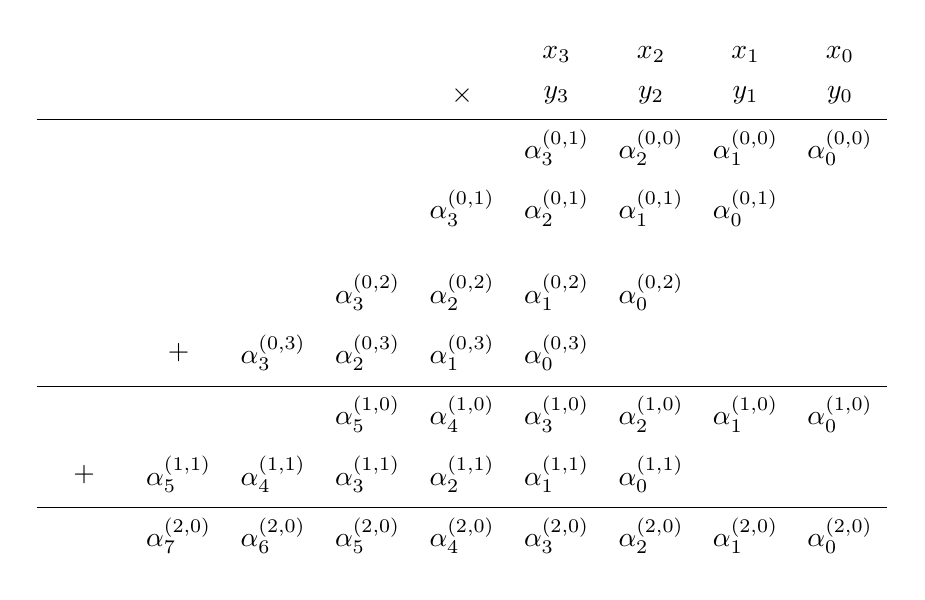
\begin{tikzpicture}
  \matrix (m) [
    matrix of nodes,
    nodes={anchor=center, minimum width=1.2cm},
    column sep=0pt,
    row sep=2pt
  ] {
  & & & &          &  $x_{3}$ & $x_{2}$ &  $x_1$ & $x_0$ \\
  & & & & $\times$ &  $y_{3}$ & $y_{2}$ &  $y_1$ & $y_0$ \\ \hline
  & & & &                        & $\alpha^{(0,1)}_{3}$ & $\alpha^{(0,0)}_{2}$  & $\alpha^{(0,0)}_1$ & $\alpha^{(0,0)}_0$ \\
  & & & & $\alpha^{(0,1)}_{3}$ & $\alpha^{(0,1)}_{2}$ & $\alpha^{(0,1)}_1$  & $\alpha^{(0,1)}_0$ & \\
  & \\
  &                        & & $\alpha^{(0,2)}_{3}$ & $\alpha^{(0,2)}_2$ & $\alpha^{(0,2)}_1$ & $\alpha^{(0,2)}_{0}$  \\
    & +                       & $\alpha^{(0,3)}_{3}$ & $\alpha^{(0,3)}_{2}$ & $\alpha^{(0,3)}_1$ & $\alpha^{(0,3)}_0$   \\
    \hline  & & &     $\alpha^{(1,0)}_{5}$ & $\alpha^{(1,0)}_4$ & $\alpha^{(1,0)}_{3}$ & $\alpha^{(1,0)}_{2}$  & $\alpha^{(1,0)}_1$ & $\alpha^{(1,0)}_0$\\
    + &      $\alpha^{(1,1)}_{5}$ & $\alpha^{(1,1)}_4$ & $\alpha^{(1,1)}_{3}$ & $\alpha^{(1,1)}_{2}$  & $\alpha^{(1,1)}_1$ & $\alpha^{(1,1)}_0$\\
     \hline   & $\alpha^{(2,0)}_7$ & $\alpha^{(2,0)}_{6}$ &  $\alpha^{(2,0)}_{5}$ & $\alpha^{(2,0)}_4$ & $\alpha^{(2,0)}_{3}$ & $\alpha^{(2,0)}_{2}$  & $\alpha^{(2,0)}_1$ & $\alpha^{(2,0)}_0$\\
  };
\end{tikzpicture}
\end{center}
\end{widetext}
\caption{Explicit multiplication of $4$-bit integers. According to Claim 2, each partial sum has at most $n+2^d$ bits, with a possibility of leading zeros.}
\label{fig:exp_mult}
\end{figure*}

\begin{comment}
\begin{center}
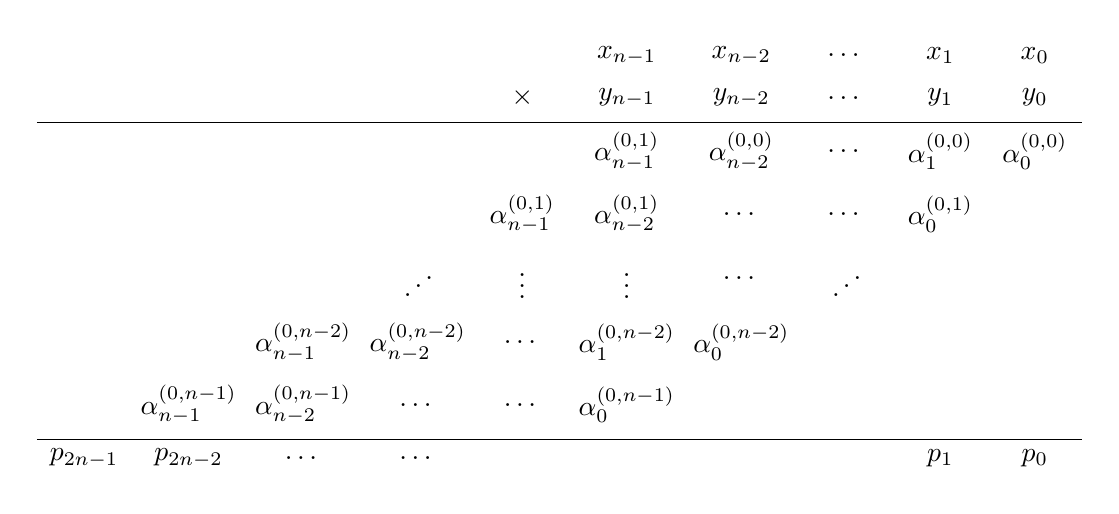
\begin{tikzpicture}
  \matrix (m) [
    matrix of nodes,
    nodes={anchor=center, minimum width=1.2cm},
    column sep=0pt,
    row sep=2pt
  ] {
  & & & &          &  $x_{n-1}$ & $x_{n-2}$ & $\dots$ & $x_1$ & $x_0$ \\
  & & & & $\times$ &  $y_{n-1}$ & $y_{n-2}$ & $\dots$ & $y_1$ & $y_0$ \\ \hline
  & & & &                        & $\alpha^{(0,1)}_{n-1}$ & $\alpha^{(0,0)}_{n-2}$ & $\dots$ & $\alpha^{(0,0)}_1$ & $\alpha^{(0,0)}_0$ \\
  & & & & $\alpha^{(0,1)}_{n-1}$ & $\alpha^{(0,1)}_{n-2}$ & $\dots$ & $\dots$ & $\alpha^{(0,1)}_0$ & \\
  & & & $\iddots$ & $\vdots$ & $\vdots$ & $\dots$ & $\iddots$ & & \\ 
  &                        & $\alpha^{(0,n-2)}_{n-1}$ & $\alpha^{(0,n-2)}_{n-2}$ & $\dots$ & $\alpha^{(0,n-2)}_1$ & $\alpha^{(0,n-2)}_0$ \\
  & $\alpha^{(0,n-1)}_{n-1}$ & $\alpha^{(0,n-1)}_{n-2}$ & $\dots$ & $\dots$ & $\alpha^{(0,n-1)}_0$ & \\
    \hline $p_{2n-1}$ & $p_{2n-2}$ & $\dots$ & $\dots$ &
    & & & &
    $p_1$ & $p_0$ \\
  };
\end{tikzpicture}
\end{center}

\newcommand{\threemat}[3]{\ensuremath{\left[\begin{smallmatrix}{#1}\vspace{0.1cm}\\{#2}\vspace{0.1cm}\\{#3}\end{smallmatrix}\right]}}

\begin{center}
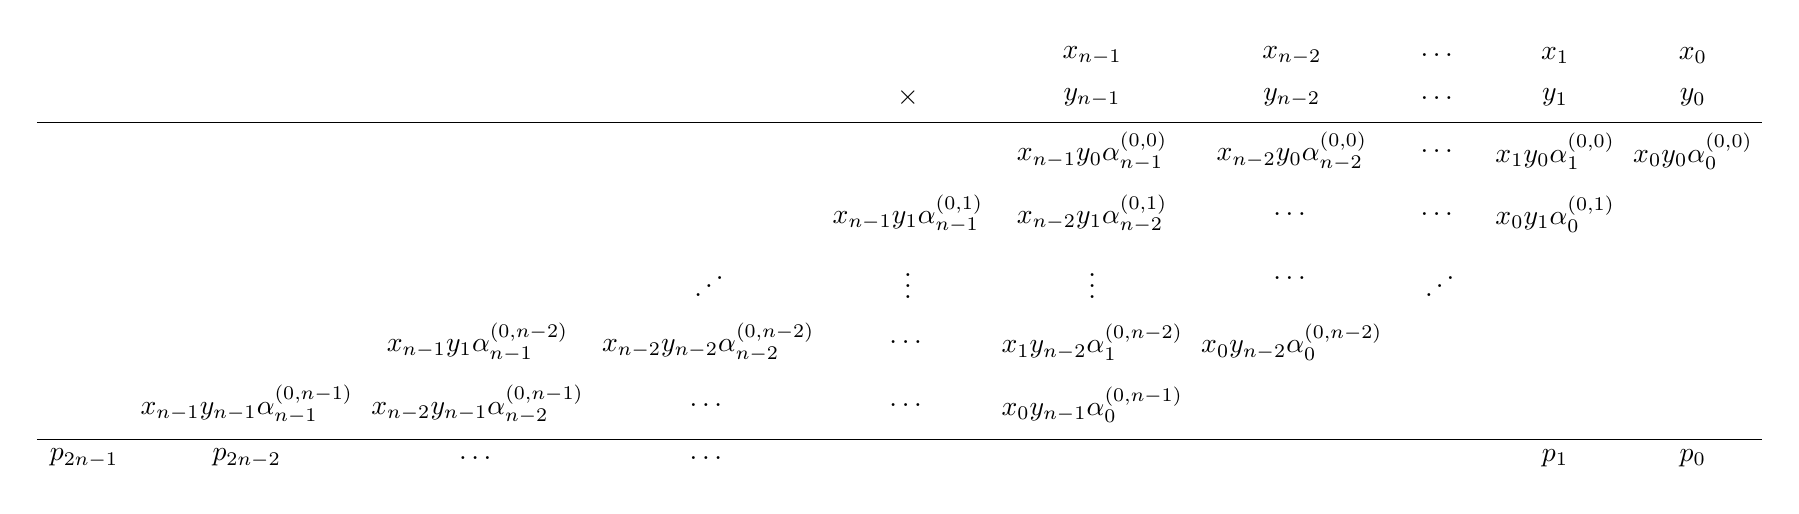
\begin{tikzpicture}
  \matrix (m) [
    matrix of nodes,
    nodes={anchor=center, minimum width=1.2cm},
    column sep=0pt,
    row sep=2pt
  ] {
  & & & &          &  $x_{n-1}$ & $x_{n-2}$ & $\dots$ & $x_1$ & $x_0$ \\
  & & & & $\times$ &  $y_{n-1}$ & $y_{n-2}$ & $\dots$ & $y_1$ & $y_0$ \\ \hline
  & & & &                        & $\threemat{x_{n-1}}{y_0}{\alpha^{(0,0)}_{n-1}}$ & $\threemat{x_{n-2}}{y_0}{\alpha^{(0,0)}_{n-2}}$ & $\dots$ & $\threemat{x_1}{y_0}{\alpha^{(0,0)}_1}$ & $\threemat{x_{0}}{y_0}{\alpha^{(0,0)}_0}$ \\
  & & & & $\threemat{x_{n-1}}{y_1}{\alpha^{(0,1)}_{n-1}}$ & $\threemat{x_{n-2}}{y_1}{\alpha^{(0,1)}_{n-2}}$ & $\dots$ & $\dots$ & $\threemat{x_{0}}{y_1}{\alpha^{(0,1)}_0}$ & \\
  & & & $\iddots$ & $\vdots$ & $\vdots$ & $\dots$ & $\iddots$ & & \\ 
  &                        & $\threemat{x_{n-1}}{y_1}{\alpha^{(0,n-2)}_{n-1}}$ & $\threemat{x_{n-2}}{y_{n-2}}{\alpha^{(0,n-2)}_{n-2}}$ & $\dots$ & $\threemat{x_{1}}{y_{n-2}}{\alpha^{(0,n-2)}_1}$ & $\threemat{x_{0}}{y_{n-2}}{\alpha^{(0,n-2)}_0}$ \\
  & $\threemat{x_{n-1}}{y_{n-1}}{\alpha^{(0,n-1)}_{n-1}}$ & $\threemat{x_{n-2}}{y_{n-1}}{\alpha^{(0,n-1)}_{n-2}}$ & $\dots$ & $\dots$ & $\threemat{x_{0}}{y_{n-1}}{\alpha^{(0,n-1)}_0}$ & \\
    \hline $p_{2n-1}$ & $p_{2n-2}$ & $\dots$ & $\dots$ &
    & & & &
    $p_1$ & $p_0$ \\
  };
\end{tikzpicture}
\end{center}

\end{comment}

\begin{comment}
Our goal is to perform the following operation:

\begin{align*}
    &\ket{z^{(0)}}\otimes\ket{z^{(1)}}\otimes\dots\otimes\ket{z^{(n-1)}}\\ 
    &\rightarrow \dots\ket{z^{(0)}+\dots+z^{(n-1)}}\dots
\end{align*}

Note that we don't care about the other results other than $\ket{z^{(1)}+z^{(2)}+\dots+z^{(n)}}$ in the output. We also note that we can make the ancillary registers have some size that is a constant multiple of $n$ such that they will all be large enough to store the total sum.\\
\end{comment}







\begin{figure}[h]
    \centering
    \begin{quantikz}[column sep=0.45cm]
        \lstick{$\ket{\alpha^{(0,0)}}$} &  \gate[3]{\texttt{\;\;Add}_1}\gateinput{0} & \qw                     & \qw &\qw &\rstick{$\ket{\alpha^{(0,0)}}$}\\
        \lstick{$\ket{\alpha^{(0,1)}}$} &\gateinput{1}      & \qw   & \qw &\qw &\rstick{$\ket{\alpha^{(0,1)}}$}\\
        \lstick{$\ket{0}^{\otimes 6}$} &\gateinput{2}     & \qw   & \gate[5]{\texttt{Add}_2}\gateinput{0} &\qw &\rstick{$\ket{\alpha^{(1,0)}}$}\\
        \lstick{$\ket{\alpha^{(0,2)}}$} &  \gate[3]{\texttt{\;\;Add}_1}\gateinput{0}  & \qw & \qw &\qw &\rstick{$\ket{\alpha^{(0,2)}}$}\\
        \lstick{$\ket{\alpha^{(0,3)}}$} & \gateinput{1}  & \qw      & \qw &\qw &\rstick{$\ket{\alpha^{(0,3)}}$}\\
        \lstick{$\ket{0}^{\otimes 6}$} &\gateinput{2}      & \qw   & \gateinput{1} &\qw &\rstick{$\ket{\alpha^{(1,1)}}$}\\
        \lstick{$\ket{0}^{\otimes 8}$} &\qw      & \qw   & \gateinput{2} &\qw &\rstick{$\ket{\alpha^{(2,0)}}$}
    \end{quantikz}
    \caption{$4$-bit integer Parallel Adder Tree Example.}
    \label{fig:adder_tree}
\end{figure}

\subsubsection{Efficient Parallel Adder Tree Uncomputation}\label{subsec:efficient_uncompute}

As mentioned in the introduction, this work uses clean ancillas, and so each submodule needs to be uncomputed. This subsection provides an efficient approach to uncompute ancillas corresponding to intermediate partial sums produced by the \texttt{parallel\_adder\_tree}.
% partial sums produced by the \texttt{parallel\_adder\_tree}, except for the final product.


As shown in Fig.~\ref{fig:adder}, each adder leaves its input registers unchanged. Furthermore, each adder at level $d$ requires only the partial sums produced at level $d-1$ as inputs. Consequently, all partial sums produced at levels $< d-1$ are no longer required by the \texttt{parallel\_adder\_tree}.

Using this fact, our uncomputation procedure proceeds as follows. Beginning at $d = 3$, the adders at level $d-2$ are uncomputed concurrently with the computation of the partial sums at level $d$. Because the input registers of every adder remain unchanged throughout the computation, the outputs produced during the forward pass can be reset to $\ket{0}$ by applying the inverse of the corresponding QCLA adder. This process continues until all partial sums have been uncomputed, except for the final adder whose output register stores the result.

Uncomputing a QCLA is equivalent to reversing the circuit and therefore uses no more gates, ancillary qubits, or circuit depth than the original adder. As a result, the asymptotic resource costs of the \texttt{parallel\_adder\_tree} are preserved.


This uncomputation procedure doubles the total gate count of the adder tree. However, the circuit depth and Toffoli depth increase by only one layer. Indeed, once the computation process begins at $d=3$, each level simultaneously computes level $d$ and uncomputes level $d-2$, except for the final level, which is not uncomputed. The ancillary qubit cost is more involved and will be discussed in the next subsection.

\subsubsection{Qubit-Efficient Parallel Adder Tree}\label{subsec:efficient_adder}

For $n$-qubit addition, the original QCLA uses at most $n$ ancillary qubits for computation and is designed such that these qubits are reset to $\ket{0}$ at the end of the adder \cite{Draper2004}. We exploit this property to reuse ancillas across layers of the tree. As will be discussed in the next section, the \texttt{fast\_copy} procedure is uncomputed before the start of the \texttt{parallel\_adder\_tree}, freeing up $2n^2$ ancillary qubits. In this subsection, we will show that these $2n^2$ qubits are sufficient for this submodule, so no additional ancillary qubits are required.

% \begin{claim}
%     The \texttt{parallel\_adder\_tree}, including all uncomputation steps, requires fewer than $2n^2$ ancillary qubits.
% \end{claim}
% \begin{proof}
We analyze the qubit usage level-by-level, accounting for both the computational ancillas used by the adders and the registers storing the partial sums.

\paragraph{Forward computation.}
We first consider only the production of partial sums. It is sufficient to analyze the \texttt{overlapping\_sum} stage of the adder, since this stage will use and uncompute $n$ computational ancilla qubits. Throughout the \texttt{parallel\_adder\_tree}, the \texttt{carry\_propagation} acts on a prefix of size at most $2^{\log{n}-1} = \frac{n}{2}$. In the worst case, which occurs at level $\log{n}$, this stage requires $\frac{n}{2}$ qubits for computation and another $\frac{n}{2}$ qubits to store the output. Therefore, the $n$ ancillas reused from the \texttt{overlapping\_sum} stage are sufficient for this stage as well.


Each adder at level $d$ outputs a partial sum stored in a register of size $n+2^d$ qubits. By the property of a binary tree, there are $\lceil n/2^d\rceil$ adders at level $d$, and so the total number of qubits required to store the outputs at this level is at most
\begin{align}
\frac{n^2}{2^d} + n.
\end{align}
Each adder in the \texttt{overlapping\_sum} stage takes $n$ qubits of inputs and requires $n$ computational ancillary qubits. So, the number of computational ancillas required at level $d$ is at most
\begin{align}
\frac{n^2}{2^d}.
\end{align}
These ancillas are released at the end of the level and reused in level $d+1$.

At level $d=1$, no qubits are available for reuse, so the total number of ancillas required is
\begin{align}
n^2 + n.
\end{align}
For each level $d\ge 2$, the ancillas from the previous level are reused, so the additional number of qubits required is
\begin{align}
\frac{n^2}{2^{d}} + n +\frac{n^2}{2^{d}}  - \frac{n^2}{2^{d-1}} = n.
\end{align}
Thus, for any $d \in [1,\lceil \log n\rceil]$, the total number of ancillas required to produce partial sums up to level $d$ is
\begin{align}
    n^2 + dn
    \label{eq:sum_qubits_rewrite}
\end{align}

\paragraph{Uncomputation.}
We now incorporate the uncomputation of the ancillas containing the intermediate partial sums. 
Uncomputing an adder is equivalent to running it in reverse. Since the input registers of each adder remain unchanged throughout the computation, the outputs produced during the forward pass can be reset to $\ket{0}$ by applying the inverse of the corresponding QCLA circuit. This releases both the computational ancillas and the output register associated with that adder.

At level $d \ge 3$, the circuit simultaneously (i) computes the partial sums at level $d$ and (ii) uncomputes the adders from level $d-2$. The forward computation at level $d$ requires at most
\begin{align}
\frac{n^2}{2^{d-1}} + n 
\end{align}
ancillary qubits (output registers plus computational ancillas), while the uncomputation of level $d-2$ requires at most
\begin{align}   
\frac{n^2}{2^{d-2}}
\end{align}
computational ancillas.

On the other hand, uncomputing level $d-2$ frees
\begin{align}
\frac{n^2}{2^{d-3}} + n 
\end{align}
qubits (both the stored partial sums and the computational ancillas of that level). The net change in the number of qubits in use when moving from level $d-1$ to level $d$ is
\begin{align}
&n
- \left(\frac{n^2}{2^{d-3}} + n + \frac{n}{2^{d-2}}\right)  < 0.
\end{align}
Hence, for every $d > 3$, the total number of qubits in use strictly decreases.


Consequently, the maximum number of ancillas in use occurs among the first three levels. Using \eqref{eq:sum_qubits_rewrite}, we obtain
\begin{align}
    d=1&: n^2+n\\
    d=2&: n^2+2n,
\end{align}
% \[
% d=1:\quad n^2 + n,
% \]
% \[
% d=2:\quad n^2 + 2n,
% \]
and for level $d=3$, we also uncompute level $1$, which costs $\frac{n^2}{2}$ ancillas. Hence, the total number of ancillas in use at level $3$ is
\begin{align}
    n^2 + 3n + \frac{n^2}{2}
    &= \frac{3}{2}n^2 + 3n \\
    &\le 2n^2,
\end{align}
where the final inequality holds for all $n\ge 6$ (and smaller $n$ can be handled by adding a constant number of ancillas).

Since the qubit usage decreases for all subsequent levels, the total number of ancillary qubits required by the \texttt{parallel\_adder\_tree}, including uncomputation, is strictly less than $2n^2$.
% \end{proof}

\subsubsection{Depth and Size Analysis}\label{subsec:gate_opt_adder}

In this section, we analyze the depth and gate cost of the \texttt{parallel\_adder\_tree}. We consider the contribution of each stage of the modified adder.

Consider the adder at depth $d$, with inputs $\ket{\alpha^{(d-1,2r)}}, \ket{\alpha^{(d-1,2r+1)}}$. As mentioned earlier, the \texttt{suffix\_copying} stage can be implemented by reusing the least significant $2^{d-1}$ qubits of $\ket{\alpha^{(d-1,2r)}}$, and so it does not incur any depth or size cost. 

The \texttt{overlapping\_sum} stage is an $n$-qubit QCLA instance, which is known to have a depth of at most $2\log{n}+7$, Toffoli depth at most $2\log{n}+4$, and uses at most $5n-3\log{n}$ Toffoli gates, $8n-3\log{n}$ gates \cite{Draper2004}. There are $2n$ adders in total (including uncomputation). Thus, the Toffoli count is 
\begin{align}10n^2-6n\log{n},\end{align}
and the total gate count is 
\begin{align}16n^2-6n\log{n}.\end{align}
The total depth contribution of this stage is equivalent to having $\lceil\log{n}\rceil+1$ layers, as discussed in Sec.~\ref{subsec:efficient_uncompute}. So, the depth is 
\begin{align}
    2\log^2{n}+9\log{n}+7,
\end{align}
and the total Toffoli depth is
\begin{align}
    2\log^2{n}+6\log{n}+4.
\end{align}


The \texttt{carry\_propagation} stage also uses the QCLA, but its size depends on the depth of the adder. At depth-level $d$, the input size to the adder is $2^{d-1}$, and so this adder has circuit depth of at most $2d+5$, Toffoli depth at most $2d+2$, and uses at most $5\cdot2^{d-1}-3(d-1)$ Toffoli gates and $8\cdot2^{d-1}-3(d-1)$ gates.


Following the discussion on circuit depth in Sec.~\ref{subsec:efficient_uncompute}, the total Toffoli depth of this stage (including uncompuation) is calculated as:
\begin{align}
    4+6+\sum_{d=1}^{\log{n}-1}(2d+2) &= \log^2{n}+\log{n} +8
\end{align}
Similarly, the depth of this circuit is:
\begin{align}
 7+9+\sum_{d=1}^{\log{n}-1}(2d+5)
    = \log^2{n} + 4\log{n}+11
\end{align}

At each depth $d$, there are $2\cdot \frac{n}{2^{d}} = \frac{n}{2^{d-1}}$ instances of the \texttt{carry\_propagation} stage (factor of 2 because of uncomputation), and each is a QCLA with input size $2^{d-1}$ qubits. Thus, the Toffoli count is at most:
\begin{align}
\sum_{d=1}^{\log{n}}(\frac{n}{2^{d-1}}(5\cdot2^{d-1}-3(d-1)))
    \leq\sum_{d=1}^{\log{n}}(5n) = 5n\log{n}
\end{align}
Similarly, the total gate count is at most $8n\log{n}$.

Putting the three stages together, the 
total Toffoli depth is $3\log^2{n}+7\log{n}+12$, 
total depth is $3\log^2{n}+13\log{n}+18$, and the 
Toffoli count and total gate count are at most $10n^2-n\log{n}$ and $16n^2+2n\log{n}$, respectively.


\begin{comment}
% It is now useful to prove the qubit requirement claim from Sec.~\ref{subsec:math}
% \begin{claim}
%     Each register $\ket{\alpha^{(d,r)}}$ can be stored using at most $n + 2^d$ qubits.
% \end{claim}

% \begin{proof}
% First, we have that all $\ket{\alpha^{(d=0,r)}}$ are stored using n qubits, which is less than $n+2^0$.
% For general $d \geq 0$, Equation~(7) shows that
% \[ \ket{\alpha^{(d,r)}}  = \ket{\alpha^{(0,r2^d)} + 2\,\alpha^{(0,r2^d+1)} + \cdots + 2^{2^d-1}\alpha^{(0,r2^d + 2^d - 1)}}. \]
% By definition of partial sum, this quantity is equal to the product of the $n$-bit integer $x$ with a $2^d$-bit substring of $y$ (specifically, the bits $y_{r2^d}, \dots, y_{r2^d+2^d-1}$). 
% The product of an $n$-bit integer and an $m$-bit integer has bit-length at most $n + m$. Taking $m = 2^d$, it follows that the value encoded in $\ket{\alpha^{(d,r)}}$ requires at most $n + 2^d$ qubits.
% \end{proof}
% Using this fact, we are able to reduce the gate cost of the parallel adder tree.
In this section we show that \texttt{parallel\_adder\_tree} has a Toffoli count
of at most $5n^2 + 2n\log{n}$ and a total gate cost of at most $8n^2 + 5n\log{n}$.

% As discussed in Sec.~\ref{subsec:math}, $\ket{\alpha^{(d,r)}}$, is a register with $n+2^d$ qubits. 
% So at each layer $d\in[1,\lceil\log{n}\rceil]$ the adder outputs $\ket{\alpha^{(d,r)}}$, which requires $n+2^d$ qubits to store.



% First, we begin with the suffix copying. To produce state $\ket{\alpha^{(d,r)}}$, the adder takes as inputs
% $\ket{\alpha^{(d-1,2r)}}$ and $\ket{\alpha^{(d-1,2r+1)}}$ and performs 
% \begin{align}
%   \ket{\alpha^{(d,r)}} = \ket{\alpha^{(d-1,2r)} + 2^{2^{(d-1)}}\alpha^{(d-1,2r+1)}}.
% \end{align}. This means the least significant $2^{d-1}$ qubits of $\ket{\alpha^{(d-1,2r)}}$
% don't have a counterpart to sum with; it can directly be used as the first
% $2^{d-1}$ qubits of the output register. In other words, we can ignore the addition involving trailing zeros.





This result reduces the input size to each QCLA in the adder tree to just $n+1$
qubits. To provide a closed-form expression for the total gate cost, we use the
result that a QCLA adder with two $n+1$-qubit inputs has Toffoli cost of at most
$5(n+1)-3\log{(n+1)}$ and total gate cost of at most $8(n+1) - 3\log{(n+1)}$.
There are a total of $n$ adders in the parallel adder tree:
\begin{align}
    &\sum_{d=1}^{\lceil\log{n}\rceil}{\frac{n}{2^d}} = n
\end{align}
and each has input size $n+1$. Thus, for the parallel adder tree, the Toffoli cost is at most 
\begin{align}
    n(5n-3\log{(n+1)}+5)&\leq 5n^2-3n\log{n} + 5n
\end{align}
and the total gate cost is at most
\begin{align}
   n(8n-3\log{(n+1)}+8)\leq 8n^2-3n\log{n} + 8n  
\end{align}

\end{comment}

\section{Fast Quantum Multiplication Algorithm}

In this section, we combine the submodules introduced in Section~\ref{sec:prelim} to construct the Fast Quantum Multiplication Algorithm. We also provide a concrete analysis of its resource costs.

\begin{algorithm}[H]
\caption{fast\_quantum\_multiplication\_algorithm}
\label{algo:multiplication}

\KwIn{
$\ket{x}\ket{y}\ket{0}^{\otimes 2n}\ket{0}^{\otimes 3n^2-2n}$
}
\vspace{0.5em}
\texttt{fast\_copy($\ket{x},\ket{y}$)}\;
\vspace{0.5em}
\texttt{partial\_products($\ket{y^{(i)}}, \ket{x^{(i)}},\ket{0^{(i)}}$)}\;

\vspace{0.5em}
\texttt{uncompute fast\_copy$(\ket{x}, \ket{y})$}\;
\vspace{0.5em}

\texttt{parallel\_adder\_tree$(\ket{\alpha^{(0,0)}}\dots\ket{\alpha^{(0,n-1)}})$}\;
\vspace{0.5em}
\texttt{redo fast\_copy$(\ket{x},\ket{y})$}\;
\vspace{0.5em}
\texttt{uncompute partial\_products($\ket{y^{(i)}}, \ket{x^{(i)}},\ket{0^{(i)}}$)}\;
\vspace{0.5em}
\texttt{uncompute fast\_copy$(\ket{x}, \ket{y})$}\;
\vspace{0.5em}

\KwOut{$\ket{x}\ket{y}\ket{xy}\ket{0}^{\otimes 3n^2-2n}$}
\end{algorithm}


\begin{claim}
    Given inputs $\ket{x}\ket{y}\ket{0}^{\otimes 2n}\ket{0}^{\otimes 3n^2-2n}$ for $n$-bit integers $x$ and $y$, Algorithm~\ref{algo:multiplication} outputs  $\ket{y}\ket{x}\ket{xy}\ket{0}^{\otimes 3n^2-2n}$ in $O(\log^2n)$ time. 
\end{claim}
\begin{proof}
    We start with initial state $\ket{x}\ket{y}\ket{0}^{\otimes 3n^2}$. \\
    
    \paragraph{Step 1: Fast Copy of $\ket{x}$ and $\ket{y}$}
    We apply Algorithm~\ref{algo:fastcopy}, \texttt{fast\_copy}, to produce $n$ copies of $\ket{x}$ and $\ket{y}$ in $O(\log n)$ time. In total, we create $n$ copies of $\ket{x}$ and $n$ copies of $\ket{y}$, resulting in the state
    \begin{align}
    \ket{x}\ket{y}\ket{y^{(0)}}\dots\ket{y^{(n-1)}}\ket{x^{(0)}}\dots\ket{x^{(n-1)}}\ket{0}^{\otimes n^2} .
    \end{align}\\   

    \paragraph{Step 2: Compute all Partial Products}
    Given $n$ copies of $\ket{x}$ and $\ket{y}$, Algorithm~\ref{algo:itwopowermultiples} performs the transformation:
    \begin{align}
        \ket{x}\ket{y}\bigotimes_{i=0}^{n-1}\smallket{y^{(i)}}\smallket{x^{(i)}}\ket{0}
        \;\longmapsto\;
        \ket{x}\ket{y}\bigotimes_{i=0}^{n-1}\smallket{y^{(i)}}\smallket{x^{(i)}}\smallket{\alpha^{(0,i)}}    
    \end{align}
    in $O(1)$ time. Each of the $n$ partial products takes $n$ qubits to store, so we require $n^2$ ancillary qubits for this step.\\
    
    \paragraph{Step 3: Uncompute Step 1}
    This step simply frees up ancilla qubits to be used for the next step. Since we didn't create any entanglement and only used CNOTs, we are able to uncompute Algorithm~\ref{algo:fastcopy} using Algorithm~\ref{algo:fastcopy} in $O(\log{n})$ time. Our state is now:
    \begin{align}
        \ket{x}\ket{y}\big(\bigotimes_{i=0}^{n-1}\smallket{\alpha^{(0,i)}}\big)\ket{0}^{\otimes 2n^2} 
    \end{align}\\

    \paragraph{Step 4: Sum of Partial Products}

    We now perform the \texttt{parallel\_adder\_tree} on all the partial products computed from the previous step, namely those of the form $\ket{\alpha^{(0,i)}} \equiv \ket{y^{(i)}x^{(i)}}$. The \texttt{parallel\_adder\_tree} algorithm from Subsection~\ref{subsec:add} maps the sum of all inputs into one register. After performing this module, we have a register containing the state:
    \begin{align}
        \ket{\alpha^{(\lceil\log{n}\rceil,0)}} = \ket{y_02^0x+y_12^1x+\dots+y_{n-1}2^{n-1}x} = \ket{xy}.
    \end{align}

    This submodule also resets all intermediate partial products to $\ket{0}$. As discussed in Section~\ref{subsec:add}, this entire submodule requires $O(\log^2{n})$ depth and $< 2n^2$ ancilla qubits, which are reused from the previous step. Following this step, we have the state:
    \begin{align}
        \ket{x}\ket{y}\big(\bigotimes_{i=0}^{n-1}\smallket{\alpha^{(0,i)}}\big)\ket{xy}\ket{0}^{\otimes 2n^2-2n} 
    \end{align}\\

    \paragraph{Step 5: Restore Copies of $\ket{x}$ and $\ket{y}$}
    To efficiently uncompute Step 2, we recreate $n$ copies of $\ket{x}$ and $\ket{y}$ by reapplying \texttt{fast\_copy}. The required $2n^2-2n$ ancillas are reused from Step 4, and the operation takes $O(\log n)$ time. Our state is now:
    \begin{align}
        \ket{x}\ket{y}\smallket{x^{(1)}}\dots\smallket{x^{(n-1)}}\smallket{y^{(1)}}\dots\smallket{y^{(n-1)}}\big(\bigotimes_{i=0}^{n-1}\smallket{\alpha^{(0,i)}}\big)\ket{xy}
    \end{align}\\

    \paragraph{Step 6: Uncompute Partial Products}
    We now apply the inverse of Algorithm~\ref{algo:itwopowermultiples}. Since the registers $\ket{y^{(i)}}$ and $\ket{x^{(i)}}$ have been restored in Step 5, we can uncompute all partial products $\ket{\alpha^{(0,i)}}$ for $i\in[0,n-1]$ in parallel, yielding the state:
    \begin{align}
        \ket{x}\ket{y}\smallket{x^{(1)}}\dots\smallket{x^{(n-1)}}\smallket{y^{(1)}}\dots\smallket{y^{(n-1)}}\ket{xy}\ket{0}^{\otimes n^2}
    \end{align}\\

    \paragraph{Step 7: Uncompute the Copies}
    Finally, we uncompute the copied registers using the inverse of \texttt{fast\_copy}, in $O(\log{n})$ depth, restoring all ancillary registers to $\ket{0}$. The final state is therefore
    \begin{align}
        \ket{y}\ket{x}\ket{xy}\ket{0}^{\otimes 3n^2-2n}.
    \end{align}

    
    It is apparent that the highest-depth step in this algorithm is Step 4, the \texttt{parallel\_adder\_tree}, which has a depth of $O(\log^2n)$.
    \end{proof}
    
    \begin{table*}[t]
    \centering
        \caption{Concrete upper-bounded resource costs for each component of the Fast Quantum Multiplication Algorithm.}
    \resizebox{\textwidth}{!}{
    \renewcommand{\arraystretch}{1.2}

    \begin{tabular}{|c|c|c|c|c|c|}
    \hline
        Algorithm Step & Depth & Toffoli depth & Toffoli Count & Gate Count & Ancillary Qubit Count\\\hline
        \texttt{fast\_copy} & $\lceil \log{n} \rceil$ & 0 & 0 & $2n^2$ & $2n^2$\\\hline
         \texttt{partial\_products} &$1$ & $1$ & $n^2$ & $n^2$ & $n^2$\\\hline
         \texttt{Undo fast\_copy} & $\lceil \log{n} \rceil$ & 0 & 0 & $2n^2$ & $-2n^2$\\\hline
         \texttt{parallel\_adder\_tree} & $3\log^2{n} +13\log{n}+18$ & $3\log^2{n} +7\log{n}+12$  & $10n^2-n\log{n}$  & $16n^2+2n\log{n}$ & $2n^2$\\\hline
        \texttt{Redo fast\_copy} & $\lceil \log{n} \rceil$ & 0 & 0 & $2n^2$ & $0$\\\hline
         \texttt{Undo partial\_products} &$1$ & $1$ & $n^2$ & $n^2$ & $0$\\\hline
         \texttt{Undo fast\_copy} & $\lceil \log{n} \rceil$ & 0 & 0 & $2n^2$ & $0$\\\hline

         Total & $3\log^2n + 17\log{n} + 20$ & $3\log^2n+7\log{n}+14$ & $12n^2-n\log{n}$ & $26n^2+2n\log{n}$ & $3n^2$\\\hline
    \end{tabular}
    }
    \label{table:results}
\end{table*}

\begin{comment}
\begin{table}[h]
    \centering
        \caption{Asymptotic resource costs for each component of the Fast Quantum Multiplication Algorithm.}
    \begin{tabular}{|c|c|c|}
    \hline
        Algorithm Step & Depth & Ancillary Qubit Count\\\hline
        \texttt{fast\_copy} & $O(\log{n})$ & $O(n^2)$\\\hline
         \texttt{partial\_products} &$O(1)$ &  $O(n^2)$\\\hline
         \texttt{Undo fast\_copy} & $O(\log{n})$ & $-O(n^2)$\\\hline
         \texttt{parallel\_adder\_tree} & $O(\log^2{n})$  & $O(n^2)$\\\hline
         Total & $O(\log^2n)$  & $O(n^2)$\\\hline
    \end{tabular}

    \label{table:results_asymp}
\end{table}
\end{comment}


\subsection{Concrete Resource Costs}

In this subsection, we analyze the resource costs of each component of Algorithm~\ref{algo:multiplication}. A summary of these costs is presented in Table~\ref{table:results}.

\begin{itemize}
\item \textbf{Step 1, \texttt{fast\_copy}: }We require a CNOT from every source qubit to every target qubit. In total, this procedure produces $n$ copies of the $n$-qubit registers $\ket{x}$ and $\ket{y}$, so we need a total of $2n^2$ CNOT gates. To store the copied registers, we need $2n^2$ ancilla qubits. As mentioned in Subsection~\ref{subsec:fast_copy}, and using the fact that the copying of $\ket{x}$ and $\ket{y}$ are indepenent, this procedure has a depth of $\log{n}$.

\item \textbf{Step 2, \texttt{partial\_products}: }Each partial product requires $n$ qubits to store, so we need a total of $n^2$ ancillary qubits. Furthermore, each call uses $n$ Toffoli gates, so \texttt{partial\_products} has a $T$-count of $n^2$, but all calls can be performed in parallel, so the Toffoli depth is $1$.

\item \textbf{Step 3, \texttt{uncompute fast\_copy}: }Similar to line 1, this procedure has depth of $\log{n}$ and requires $2n^2$ CNOT gates. However, we free up $2n^2$ qubits for later use.

\item \textbf{Step 4, \texttt{parallel\_adder\_tree}: }
This function is implemented using Draper’s out-of-place QCLA \cite{Draper2004}. From Subsec.~\ref{subsec:efficient_adder}, the adder tree requires at most $2n^2$ ancillary qubits, which can be entirely reused from the $2n^2$ qubits freed in the previous step.

From Subsec.~\ref{subsec:gate_opt_adder}, 
the depth is 
$3\log^2{n}+13\log{n}+18$, Toffoli depth is $3\log^2{n}+7\log{n}+12$, 
Toffoli count is at most 
$10n^2 -n\log n$, and the total gate count is at most 
$16n^2 +2n\log n$. 


\item \textbf{Step 5, \texttt{redo fast\_copy}: }As in Step 1, this operation requires $2n^2$ CNOT gates and has depth $\lceil \log n \rceil$. The $2n^2$ ancilla qubits required can be reused from the previous step.

\item \textbf{Step 6, \texttt{uncompute partial\_products}: }No additional ancillary qubits are required, since this step reverses Step 2. The operation requires $n^2$ Toffoli gates and has Toffoli depth $1$.

\item \textbf{Step 7, \texttt{uncompute fast\_copy}: } Equivalent to Step 3, this procedure has depth $\lceil \log n \rceil$ and requires $2n^2$ CNOT gates.
\end{itemize}


\section{Conclusion}

Optimizing quantum algorithms for multiplication is important for its key role in many applications, such as modular exponentiation in Shor's algorithm, Hamiltonian simulation, the HHL algorithm, and Taylor series approximations \cite{Shor1997, pavlidis2013fastquantummodularexponentiation, Harrow_2009, Childs_2017, Berry_2015}. As such, improvements in the depth, gate count, and ancillary qubit usage of quantum multiplication directly lead to advancements in higher-level quantum algorithms.

In this work, we demonstrated how parallelization techniques can be leveraged to reduce the overall circuit depth and $T$-depth to $O(\log^2 n)$ while maintaining reasonable qubit overhead and gate complexity. Our construction is simple and modular, enabling straightforward implementation, analysis, and integration into larger quantum computing applications.

These optimizations are particularly significant in the fault-tolerant setting, where $T$-depth is an especially important cost function. Future work may explore further reductions in $T$-depth through improved Quantum Carry Lookahead Adder constructions, alternative parallel addition schemes, or more advanced multiplication frameworks.


\begin{acknowledgments}
The authors thank Matthew Amy, Vlad Gheorghiu, and Andrew Jena for their feedback on this manuscript.
\end{acknowledgments}
\bibliography{bib}

\end{document}
